\input{"preamble.tex"}

\addbibresource{HomologicalAlgebra.bib}

\let\Begin\begin
\let\End\end
\newcommand\wrapenv[1]{#1}

\makeatletter
\def\ScaleWidthIfNeeded{%
 \ifdim\Gin@nat@width>\linewidth
    \linewidth
  \else
    \Gin@nat@width
  \fi
}
\def\ScaleHeightIfNeeded{%
  \ifdim\Gin@nat@height>0.9\textheight
    0.9\textheight
  \else
    \Gin@nat@width
  \fi
}
\makeatother

\setkeys{Gin}{width=\ScaleWidthIfNeeded,height=\ScaleHeightIfNeeded,keepaspectratio}%

\title{
\rule{\linewidth}{1pt} \\
\textbf{
    Homological Algebra
  }
    \\ {\normalsize Lectures by Brian Boe. University of Georgia, Spring
2021} \\
  \rule{\linewidth}{2pt}
}
\titlehead{
    \begin{center}
  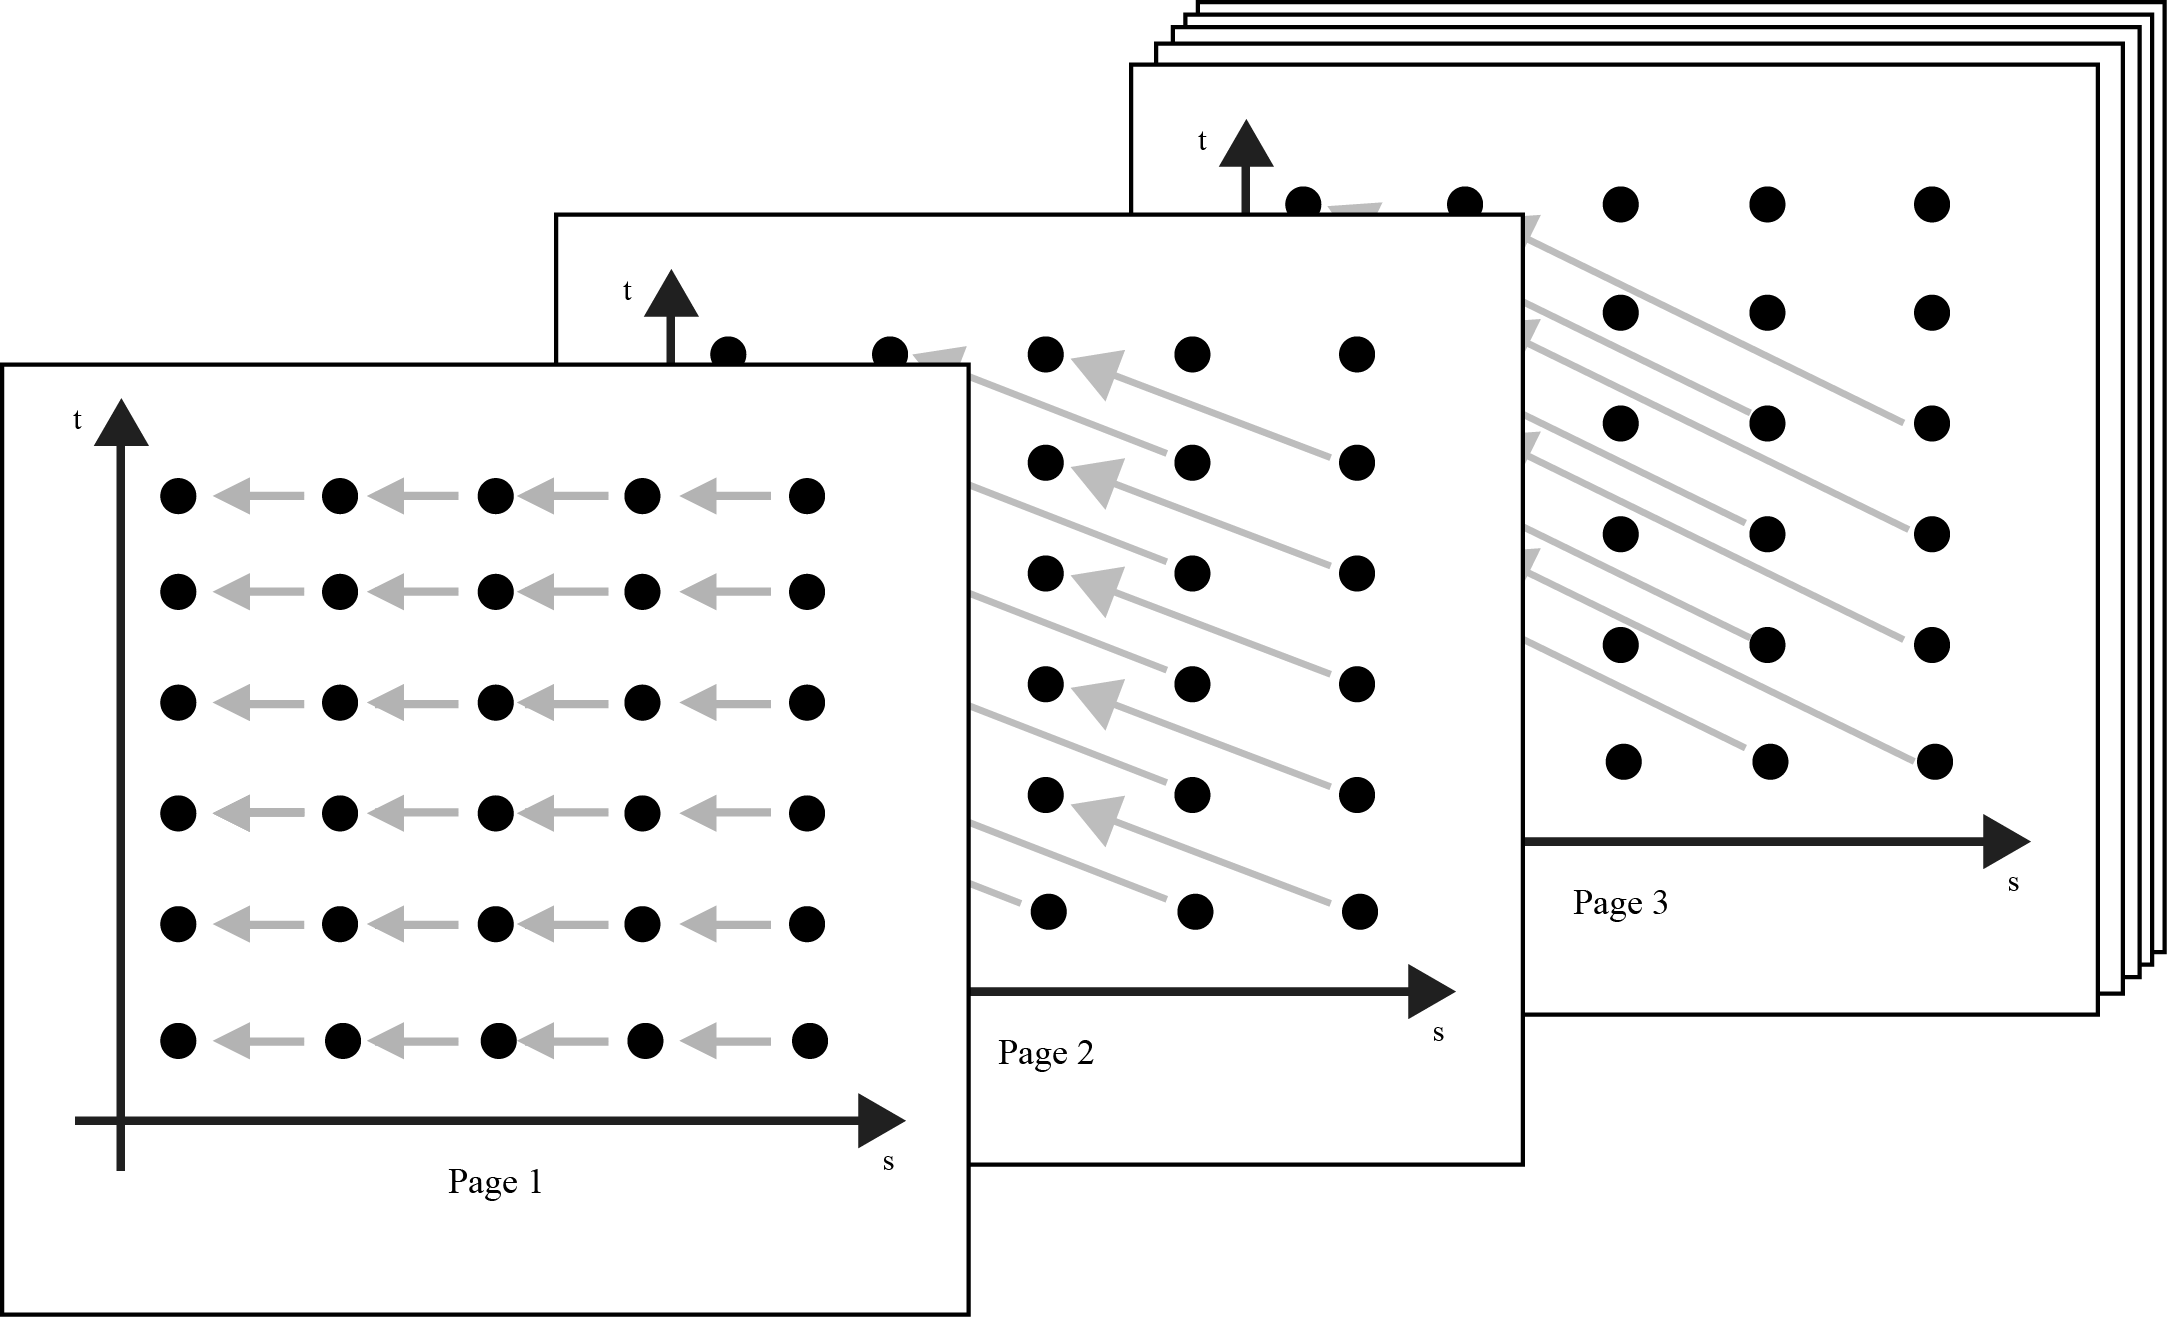
\includegraphics[width=\linewidth,height=0.45\textheight,keepaspectratio]{figures/cover.png}
  \end{center}
       \begin{minipage}{.35\linewidth}
    \begin{flushleft}
      \vspace{2em}
      {\fontsize{6pt}{2pt} \textit{Notes: These are notes live-tex'd
from a graduate course in Homological Algebra taught by Brian Boe at the
University of Georgia in Spring 2021. As such, any errors or
inaccuracies are almost certainly my own. } } \\
    \end{flushleft}
    \end{minipage}
    \hfill
    \begin{minipage}{.65\linewidth}
    \end{minipage}
  }







\begin{document}

\date{}
\author{D. Zack Garza}
\maketitle
\begin{flushleft}
\textit{D. Zack Garza} \\
\textit{University of Georgia} \\
  \textit{\href{mailto: dzackgarza@gmail.com}{dzackgarza@gmail.com}} \\
{\tiny \textit{Last updated:} 2021-01-17 }
\end{flushleft}


\newpage

% Note: addsec only in KomaScript
\addsec{Table of Contents}
\tableofcontents
\newpage

\def\contradiction
{
\tikz[baseline, x=0.2em, y=0.2em, line width=0.04em]
\draw (0,0) -- ({4*cos(45)},{4*sin(45)})
    (-1,1) -- ({-1 + 4*cos(45)},{1 + 4*sin(45)})
    (-1,3) -- ({-1 + 4*cos(315)},{3 + 4*sin(315)})
    (0,4) -- ({0 + 4*cos(315)},{4 + 4*sin(315)});
}

\hypertarget{wednesday-january-13}{%
\section{Wednesday, January 13}\label{wednesday-january-13}}

Reference:

\begin{itemize}
\item
  The course text is Charles A. Weibel, An introduction to homological
  algebra, Cambridge Studies in Advanced Mathematics 38, Cambridge
  University Press, 1994.
\item
  See corrections: Many corrections to Weibel's book:
  \url{http://www.math.rutgers.edu/~weibel/Hbook-corrections.html}
\item
  1.1-1.5, 2.2-2.7, 3.4 3.6, 6.1, 5.1-5.2, 5.4-5.8, 6.8, 6.7, 6.3,
  7.1-7.5, 7.7-7.8, along with most of Appendix A when needed.
\item
  Course Website:
  \url{https://uga.view.usg.edu/d2l/le/content/2218619/viewContent/33763436/View}
\end{itemize}

\hypertarget{overview}{%
\subsection{Overview}\label{overview}}

\begin{definition}[Exact complexes]

A \textbf{complex} is given by
\begin{align*}
\cdots \xrightarrow{d_{i-1}} M_{i-1} \xrightarrow{d_i} M_i \xrightarrow{d_{i+1}}M_{i+1} \to  \cdots
.\end{align*}
where \(M_i \in {R{\hbox{-}}\operatorname{mod}}\) and
\(d_i \circ d_{i-1} = 0\), which happens if and only if
\(\operatorname{im}d_{i-1} \subseteq \ker d_i\). If
\(\operatorname{im}d_{i-1} = \ker d_i\), this complex is \textbf{exact}.

\end{definition}

\begin{example}[?]

We can apply a functor such as \(\otimes_R N\) to get a new complex
\begin{align*}
\cdots \xrightarrow{d_{i-1} \otimes 1_N} M_{i-1} \otimes_R N \xrightarrow{d_i \otimes 1} M_i \otimes N  \to M_{i+1} \xrightarrow{d_{i+1} \otimes 1} \cdots
.\end{align*}

\end{example}

\begin{example}[?]

Applying \({\operatorname{Hom}}(N, {\,\cdot\,})\) similarly yields
\begin{align*}
{\operatorname{Hom}}_R(N, M_{i}) \xrightarrow{d_{i-1}^*} {\operatorname{Hom}}_R(N, M_{i+1})
,\end{align*}
where \(d_i^* = d_i \circ ({\,\cdot\,})\) is given by composition.

\end{example}

\begin{example}[?]

Applying \({\operatorname{Hom}}({\,\cdot\,}, N)\) yields
\begin{align*}
{\operatorname{Hom}}_R(M_i, N) \xrightarrow{d_{i}^*} {\operatorname{Hom}}_R(M_{i+1}, N)
\end{align*}
where \(d_i^* = ({\,\cdot\,}) \circ d_i\).

\end{example}

\begin{remark}

Note that we can also take complexes with arrows in the other direction.
For \(F\) a functor, we can rewrite these examples as
\begin{align*}
d_i^* \circ d_{i-1}^* = F(d_i) \circ F(d_{i-1}) = F(d_i \circ d_{i-1}) = F(0) = 0
,\end{align*}
provided \(F\) is nice enough and sends zero to zero. This follows from
the fact that functors preserve composition. Even if the original
complex is exact, the new one may not be, so we can define the
following:

\end{remark}

\begin{definition}[Cohomology]

\begin{align*}
H^i(M^*) = \ker d_i^* / \operatorname{im}d_{i-1}^*
.\end{align*}

\end{definition}

\begin{remark}

These will lead to \textbf{\(i\)th derived functors}, and category
theory will be useful here. See appendix in Weibel. For a category
\(\mathcal{C}\) we'll define

\begin{itemize}
\tightlist
\item
  \(\mathrm{Obj}(\mathcal{C} )\) as the objects
\item
  \({\operatorname{Hom}}_{\mathcal{C}}(A, B)\) a set of morphisms
  between them, where a more modern notation might be
  \(\mathrm{Mor}(A, B)\).
\item
  Morphisms compose: \(A \xrightarrow{f} B \xrightarrow{g} C\) means
  that \(g\circ f \in {\operatorname{Hom}}_{\mathcal{C}}(A, C)\)
\item
  Associativity
\item
  Identity morphisms
\end{itemize}

See the appendix for diagrams defining zero objects and the zero map,
which we'll need to make sense of exactness. We'll also needs notions of
kernels and images, or potentially cokernels instead of images since
they're closely related.

\end{remark}

\begin{remark}

In the examples, we had \(\ker d_i \subseteq M_i\), but this need not be
true since the objects in the category may not be sets. Such an example
is the category of complexes of \(R{\hbox{-}}\)modules:
\(\operatorname{Cx}({R{\hbox{-}}\operatorname{mod}})\). In this setting,
kernels will be subcomplexes but not subsets.

\end{remark}

\begin{definition}[Functors]

Recall that \textbf{functors} are ``functions'' between categories
\(F: \mathcal{C}\to \mathcal{D}\) such that

\begin{itemize}
\item
  Objects are sent to objects,
\item
  Morphisms are sent to morphisms, so
  \(A \xrightarrow{f} B \leadsto F(A) \xrightarrow{F(f)} F(B)\),
\item
  \(F\) respects composition and identities
\end{itemize}

\end{definition}

\begin{example}[Hom]

\({\operatorname{Hom}}_R(N, {\,\cdot\,}): {R{\hbox{-}}\operatorname{mod}}\to {\operatorname{Ab}}\),
noting that the hom set may not have an \(R{\hbox{-}}\)module structure.

\end{example}

\begin{remark}

Taking cohomology yields the \(i\)th derived functors of \(F\), for
example \(\operatorname{Ext}^i, \operatorname{Tor}_i\). Recall that
functors can be \emph{covariant} or contravariant. See section 1 for
formulating simplicial and singular homology (from topology) in this
language.

\end{remark}

\hypertarget{chapter-1-chain-complexes}{%
\subsection{Chapter 1: Chain
Complexes}\label{chapter-1-chain-complexes}}

\hypertarget{complexes-of-rhbox-modules}{%
\subsubsection{\texorpdfstring{Complexes of
\(R{\hbox{-}}\)modules}{Complexes of R\{\textbackslash hbox\{-\}\}modules}}\label{complexes-of-rhbox-modules}}

\begin{definition}[Exactness]

Let \(R\) be a ring with 1 and define
\({R{\hbox{-}}\operatorname{mod}}\) to be the category of \emph{right}
\(R{\hbox{-}}\)modules. \(A \xrightarrow{f} B \xrightarrow{g} C\) is
\textbf{exact} if and only if \(\ker g = \operatorname{im}f\), and in
particular \(g\circ f = 0\).

\end{definition}

\begin{definition}[Chain Complex]

A \textbf{chain complex} is
\begin{align*}
C_{\,\cdot\,}\coloneqq(C_{\,\cdot\,}, d_{\,\cdot\,}) \coloneqq\qty{ \cdots \to C_{n+1} \xrightarrow{d_{n+1}} C_n \xrightarrow{d_n} C_{n-1} \to \cdots }
\end{align*}
for \(n \in {\mathbb{Z}}\) such that \(d_n \circ d_{n+1} = 0\). We drop
the \(n\) from the notation and write \(d^2 \coloneqq d\circ d = 0\).

\end{definition}

\begin{definition}[Cycles and boundaries]

\envlist

\begin{itemize}
\tightlist
\item
  \(Z_n = Z_n(C_{\,\cdot\,}) = \ker d_n\) are referred to as
  \textbf{\(n{\hbox{-}}\)cycles}.
\item
  \(B_n = B_n(C_{\,\cdot\,}) = \operatorname{im}d_{n+1}\) are the
  \textbf{\(n{\hbox{-}}\)boundaries}.
\end{itemize}

\end{definition}

\begin{definition}[Homology of a chain complex]

Note that if \(d^2 = 0\) then \(B_n \leq Z_n \leq C_n\). In this case,
it makes sense to define the quotient module
\(H^n(C_{\,\cdot\,}) \coloneqq Z_n / B_n\), the \textbf{\(n\)th
homology} of \(C_{\,\cdot\,}\).

\end{definition}

\begin{definition}[Maps of chain complexes]

A map \(u: C_{\,\cdot\,}\to D_{\,\cdot\,}\) of chain complexes is a
sequence of maps \(u_n: C_n \to D_n\) such that all of the following
squares commute:

\begin{figure}
\centering
\resizebox{\columnwidth}{!}{%
\begin{tikzcd}
    {\cdots} & {C_{n+1}} & {C_n} & {C_{n-1}} & {\cdots} \\
    \\
    {\cdots} & {D_{n+1}} & {D_n} & {D_{n-1}} & {\cdots}
    \arrow[from=1-1, to=1-2]
    \arrow[from=1-2, to=1-3]
    \arrow[from=1-3, to=1-4]
    \arrow[from=3-1, to=3-2]
    \arrow[from=3-2, to=3-3]
    \arrow[from=3-3, to=3-4]
    \arrow[from=3-4, to=3-5]
    \arrow[from=1-4, to=1-5]
    \arrow["{u_{n+1}}", from=1-2, to=3-2]
    \arrow["{u_n}", from=1-3, to=3-3]
    \arrow["{u_{n-1}}", from=1-4, to=3-4]
\end{tikzcd}
}
\end{figure}

\end{definition}

\begin{remark}

We can thus define a category
\(\mathrm{Ch}({R{\hbox{-}}\operatorname{mod}})\) where

\begin{itemize}
\tightlist
\item
  The objects are chain complexes,
\item
  The morphisms are chain maps.
\end{itemize}

\end{remark}

\begin{exercise}[Weibel 1.1.2]

A chain complex map \(u: C_{\,\cdot\,}\to D_{\,\cdot\,}\) restricts to
\begin{align*}
u_n: Z_n(C_{\,\cdot\,}) \to Z_n(D_{\,\cdot\,}) \\
u_n: B_n(D_{\,\cdot\,}) \to B_n(D_{\,\cdot\,})
\end{align*}
and thus induces a well-defined map
\(u_{n, *}: H_n(C_{\,\cdot\,}) \to H_n(D_{\,\cdot\,})\).

\end{exercise}

\begin{remark}

Each \(H_n\) thus becomes a functor
\(\mathrm{Ch}({R{\hbox{-}}\operatorname{mod}}) \to {R{\hbox{-}}\operatorname{mod}}\)
where \(H_n(u) \coloneqq u_{*. n}\).

\end{remark}

\hypertarget{friday-january-15}{%
\section{Friday, January 15}\label{friday-january-15}}

\hypertarget{review}{%
\subsection{Review}\label{review}}

\begin{quote}
See assignment posted on ELC, due Wed Jan 27
\end{quote}

\begin{remark}

Recall that a chain complex is \(C_{\,\cdot\,}\) where \(d^2 = 0\), and
a map of chain complex is a ladder of commuting squares

\begin{quote}
\href{https://q.uiver.app/?q=WzAsMTEsWzEsMCwiQ197bi0xfSJdLFsyLDAsIkNfe259Il0sWzMsMCwiQ197bisxfSJdLFsyLDIsIkRfbiJdLFszLDIsIkRfe24rMX0iXSxbMSwyLCJEX3tuLTF9Il0sWzQsMCwiXFxidWxsZXQiXSxbNCwyLCJcXGJ1bGxldCJdLFswLDIsIlxcYnVsbGV0Il0sWzAsMCwiXFxidWxsZXQiXSxbMiwxXSxbMCw1LCJ1Il0sWzEsMywidV9uIl0sWzIsNCwidSJdLFswLDFdLFsxLDIsImRfbiJdLFs1LDNdLFszLDQsImRfbiIsMl0sWzIsNl0sWzQsN10sWzgsNV0sWzksMF1d}{Link
to diagram}

\begin{figure}
\centering
\resizebox{\columnwidth}{!}{%
\begin{tikzcd}
\cdots & {C_{n-1}} & {C_{n}} & {C_{n+1}} & \cdots \\
&& {} \\
\cdots & {D_{n-1}} & {D_n} & {D_{n+1}} & \cdots
\arrow["{u_{n-1}}", from=1-2, to=3-2]
\arrow["{u_n}", from=1-3, to=3-3]
\arrow["{u_{n+1}}", from=1-4, to=3-4]
\arrow["{d_{n-1}}", from=1-2, to=1-3]
\arrow["{d_n}", from=1-3, to=1-4]
\arrow["{d_{n-1}}", from=3-2, to=3-3]
\arrow["{d_n}"', from=3-3, to=3-4]
\arrow[from=1-4, to=1-5]
\arrow[from=3-4, to=3-5]
\arrow[from=3-1, to=3-2]
\arrow[from=1-1, to=1-2]
\end{tikzcd}
}
\end{figure}
\end{quote}

Recall that \(u_n: Z_n(C) \to Z_n(D)\) and \(u_n: B_n(C) \to B_n(D)\)
preserves these submodules, so there are induced maps
\(u_{{\,\cdot\,}, n}: H_n(D) \to H_n(D)\) where
\(H_n(C) \coloneqq Z_n(C) / B_nn-1(C)\). Moreover, taking
\(H_n({\,\cdot\,})\) is a functor from
\(\operatorname{Ch}({R{\hbox{-}}\operatorname{mod}}) \to {R{\hbox{-}}\operatorname{mod}}\)
for any fixed \(n\) and on objects \(C\mapsto H_n(C)\) and chain maps
\(u_{n} \to H_n(u) \coloneqq u_{*, n}\). Note the lower indices denote
maps going down in degree.

\end{remark}

\hypertarget{cohomology}{%
\subsection{Cohomology}\label{cohomology}}

\begin{definition}[Quasi-isomorphism]

A chain map \(u:C\to D\) is a \textbf{quasi-isomorphism} if and only if
the induced map \(u_{*, n}: H^n(C) \to H^n(D)\) is an isomorphism of
\(R{\hbox{-}}\)modules.

\end{definition}

\begin{remark}

Note that the usual notion of an isomorphism in the categorical sense
might be too strong here.

\end{remark}

\begin{definition}[Cohomology]

A \textbf{cochain complex} is a complex of the form
\begin{align*}
\cdots 
\xrightarrow{d^{n-2}}  C^{n-1}
\xrightarrow{d^{n-1}}  C^{n}
\xrightarrow{d^{n}}  C^{n+1}
\cdots
\end{align*}
where \(d^n \circ d^{n-1} = 0\). We similarly write
\(Z^n(C) \coloneqq\ker d^n\) and
\(B^n(C) \coloneqq\operatorname{im}d^{n-1}\) and write the
\(R{\hbox{-}}\)module \(H^n(C) \coloneqq Z^n/B^n\) for the \(n\)th
\textbf{cohomology} of \(C\).

\end{definition}

\begin{remark}

There is a way to go back and forth bw chain complexes and cochain
complexes: set \(C_n \coloneqq C^{-n}\) and \(d_n \coloneqq d^{-n}\).
This yields
\begin{align*}
C^{-n} 
\xrightarrow{d^{-n}} 
C^{-n+1} 
\iff C_n \xrightarrow{d^n} C_{n-1}
,\end{align*}
and the notions of \(d^2 = 0\) coincide.

\end{remark}

\begin{definition}[Bounded complexes]

A cochain complex \(C\) is \textbf{bounded} if and only if there exists
an \(a\leq b \in {\mathbb{Z}}\) such that
\(C_n \neq 0 \iff a\leq n \leq b\). Similarly \(C^n\) is bounded above
if there is just a \(b\), and \textbf{bounded below} for just an \(a\).
All of the same definitions are made for cochain complexes.

\end{definition}

\begin{remark}

See the book for classical applications:

\begin{itemize}
\tightlist
\item
  1.1.3: Simplicial homology
\item
  1.1.5: Singular homology
\end{itemize}

\end{remark}

\hypertarget{operations-on-chain-complexes}{%
\subsection{Operations on Chain
Complexes}\label{operations-on-chain-complexes}}

\begin{remark}

Write \(\operatorname{Ch}\) for
\(\operatorname{Ch}({R{\hbox{-}}\operatorname{mod}})\), then if
\(f,g: C\to D\) are chain maps then \(f+g:C\to D\) can be defined as
\((f+g)(x) = f(x) + g(x)\), since \(D\) has an addition coming from its
\(R{\hbox{-}}\)module structure. Thus the hom sets
\({\operatorname{Hom}}_{\operatorname{Ch}}(C, D)\) becomes an abelian
group. There is a distinguished \textbf{zero object}\footnote{See
  appendix A 1.6 for initial and terminal objects. Note that
  \(\emptyset\) is an initial but non-terminal object in
  \({\operatorname{Set}}\), whereas zero objects are both.} \(0\),
defined as the chain complex with all zero objects and all zero maps.
Note that we also have a zero map given by the composition
\((C \to 0) \circ (0\to D)\).

\end{remark}

\begin{definition}[Products and Coproducts]

If \(\left\{{A_ \alpha}\right\}\) is a family of complexes, we can form
two new complexes:

\begin{itemize}
\item
  The \textbf{product}
  \(\qty{ \prod_ \alpha A_ \alpha}_n \coloneqq\prod_ \alpha A _{\alpha, n}\)
  with the differential
  \begin{align*}
  \qty{ \prod d_ \alpha}_n: \prod A _{\alpha, n} \xrightarrow{d _{\alpha, n}} \prod A _{\alpha, n-1}
  .\end{align*}
\item
  The \textbf{coproduct}
  \(\qty{ \coprod _{\alpha} A _{\alpha}}_n \coloneqq\bigoplus _{\alpha} A _{\alpha, n}\),
  i.e.~there are only finitely many nonzero entries, with exactly the
  same definition as above for the differential.
\end{itemize}

\end{definition}

\begin{remark}

Note that if the index set is finite, these notions coincide. By
convention, finite direct products are written as direct sums.

These structures make \(\operatorname{Ch}\) into an \textbf{additive
category}. See appendix for definition: the homs are abelian groups
where composition distributes over addition, existence of a zero object,
and existence of finite products. Note that here we have arbitrary
products.

\end{remark}

\begin{definition}[?]

We say \(B\) is a \textbf{subcomplex} of \(C\) if and only if

\begin{itemize}
\tightlist
\item
  \(B_n \leq C_n \in {R{\hbox{-}}\operatorname{mod}}\) for all \(n\),
\item
  The differentials of \(B_n\) are the restrictions of the differentials
  of \(C_n\).
\end{itemize}

\end{definition}

\begin{remark}

This can be alternatively stated as saying the inclusion \(i: B\to C\)
given by \(i_n: B_n \to C_n\) is a morphism of chain complexes. Recall
that some squares need to commute, and this forces the condition on
restrictions.

\end{remark}

\begin{definition}[Quotient Complex]

When \(B \leq C\), we can form the quotient complex \(C/B\) where
\begin{align*}
C_n/B_n \xrightarrow{\mkern 1.5mu\overline{\mkern-1.5mud_n\mkern-1.5mu}\mkern 1.5mu} C _{n-1} / B _{n-1}
.\end{align*}
Moreover there is a natural projection \(\pi: C\to C/B\) which is a
chain map.

\end{definition}

Suppose \(f:B\to C\) is a chain map, then there exist induced maps on
the levelwise kernels and cokernels, so we can form the \textbf{kernel}
and \textbf{cokernel} complex:

\begin{quote}
\href{https://q.uiver.app/?q=WzAsMTgsWzIsNCwiQ19uIl0sWzQsNCwiQ197bi0xfSJdLFsyLDIsIkJfbiJdLFs0LDIsIkJfe24tMX0iXSxbMiwwLCJcXGtlciBmX24iXSxbNCwwLCJcXGtlciBmX3tuLTF9Il0sWzIsNiwiXFxjb2sgZl9uIl0sWzQsNiwiXFxjb2sgZl97bi0xfSJdLFszLDVdLFs0LDVdLFs2LDAsIlxcY2RvdHMiXSxbNiwyLCJcXGNkb3RzIl0sWzYsNCwiXFxjZG90cyJdLFs2LDYsIlxcY2RvdHMiXSxbMCw2LCJcXGNkb3RzIl0sWzAsNCwiXFxjZG90cyJdLFswLDIsIlxcY2RvdHMiXSxbMCwwLCJcXGNkb3RzIl0sWzAsMSwiZF9uIl0sWzIsMywiZF9uIl0sWzQsNSwiXFxleGlzdHMgZF9uIiwwLHsic3R5bGUiOnsiYm9keSI6eyJuYW1lIjoiZGFzaGVkIn19fV0sWzYsNywiXFxleGlzdHMgZF9uIiwwLHsic3R5bGUiOnsiYm9keSI6eyJuYW1lIjoiZGFzaGVkIn19fV0sWzQsMiwiaV97bn0iLDFdLFsyLDAsImZfbiIsMV0sWzAsNiwiXFxwaV9uIiwxXSxbMywxLCJmX3tuLTF9IiwxXSxbMSw3LCJcXHBpX3tuLTF9IiwxXSxbNSwzLCJpX3tuLTF9IiwxXSxbMTcsNF0sWzE2LDJdLFsxNSwwXSxbMTQsNl0sWzcsMTNdLFsxLDEyXSxbMywxMV0sWzUsMTBdXQ==}{Link
to Diagram}
\end{quote}

\begin{figure}
\centering
\resizebox{\columnwidth}{!}{%
\begin{tikzcd}
    \cdots && {\ker f_n} && {\ker f_{n-1}} && \cdots \\
    \\
    \cdots && {B_n} && {B_{n-1}} && \cdots \\
    \\
    \cdots && {C_n} && {C_{n-1}} && \cdots \\
    &&& {} & {} \\
    \cdots && {\operatorname{coker}f_n} && {\operatorname{coker}f_{n-1}} && \cdots
    \arrow["{d_n}", from=5-3, to=5-5]
    \arrow["{d_n}", from=3-3, to=3-5]
    \arrow["{\exists d_n}", dashed, from=1-3, to=1-5]
    \arrow["{\exists d_n}", dashed, from=7-3, to=7-5]
    \arrow["{i_{n}}"{description}, from=1-3, to=3-3]
    \arrow["{f_n}"{description}, from=3-3, to=5-3]
    \arrow["{\pi_n}"{description}, from=5-3, to=7-3]
    \arrow["{f_{n-1}}"{description}, from=3-5, to=5-5]
    \arrow["{\pi_{n-1}}"{description}, from=5-5, to=7-5]
    \arrow["{i_{n-1}}"{description}, from=1-5, to=3-5]
    \arrow[from=1-1, to=1-3]
    \arrow[from=3-1, to=3-3]
    \arrow[from=5-1, to=5-3]
    \arrow[from=7-1, to=7-3]
    \arrow[from=7-5, to=7-7]
    \arrow[from=5-5, to=5-7]
    \arrow[from=3-5, to=3-7]
    \arrow[from=1-5, to=1-7]
\end{tikzcd}
}
\end{figure}

Here \(\ker f \leq B\) is a subcomplex, and \(\operatorname{coker}f\) is
a quotient complex of \(C\). The chain map \(i: \ker f\to B\) is a
categorical kernel of \(f\) in \(\operatorname{Ch}\), and \(\pi\) is
similarly a cokernel. See appendix A 1.6. These constructions make
\(\operatorname{Ch}\) into an \textbf{abelian category}: roughly an
additive category where every morphism has a kernel and a cokernel.

\addsec{ToDos}
\listoftodos[List of Todos]
\cleardoublepage

% Hook into amsthm environments to list them.
\addsec{Definitions}
\renewcommand{\listtheoremname}{}
\listoftheorems[ignoreall,show={definition}, numwidth=3.5em]
\cleardoublepage

\addsec{Theorems}
\renewcommand{\listtheoremname}{}
\listoftheorems[ignoreall,show={theorem,proposition}, numwidth=3.5em]
\cleardoublepage

\addsec{Exercises}
\renewcommand{\listtheoremname}{}
\listoftheorems[ignoreall,show={exercise}, numwidth=3.5em]
\cleardoublepage

\addsec{Figures}
\listoffigures
\cleardoublepage


\printbibliography[title=Bibliography]


\end{document}
